\documentclass[12pt,a4paper,oneside]{article}
\usepackage[utf8]{vietnam}
\usepackage{graphicx}
\usepackage{hyperref} 
\usepackage{fancyhdr} % used for creating header/footer
\pagestyle{fancy}

\fancyhead{}	% clean all default header/footer
\fancyfoot{}
\fancyhead[R]{Thư viện Web hỗ trợ tương tác dữ liệu đa phương tiện}
\fancyfoot[L]{Thực tập tốt nghiệp}
\fancyfoot[R] {Trang | \thepage}
\renewcommand{\headrulewidth}{0.6pt}
\renewcommand{\footrulewidth}{0pt}



\begin{document}
\tableofcontents
\newpage
\section{Giới thiệu đề tài}
\subsection{Bối cảnh}
Trực quan dữ liệu, được hiểu là cách dùng hình ảnh để biểu diễn thông tin, ngày nay đã trở nên phổ dụng bởi những lợi ích nó mang lại.

Trực quan hóa khai thác hệ thống thị giác con người để cung cấp một cách trực quan, nhanh chóng, độc lập với ngôn ngữ để xem và hiển thị dữ liệu. Đây là công cụ đắc lực để phân tích và tìm hiểu thông tin. Cho đến nay, hệ thống thị giác con người là thứ đắt nhất, trực tiếp nhất, đem lại lượng thông tin lớn nhất lưu trong bộ nhớ con người. Lượng bộ nhớ tiêu tốn để xử lý thông tin thị giác vượt xa hơn so với những giác quan khác của con người. Một số nghiên cứu ước tính rằng hệ thống thị giác của con người có thể xử lý 9 megabit thông tin trên 1 giây, tương đương với gần 1 triệu kí tự trên 1 giây.

Mặc cho tiềm năng của nó, Trực quan dữ liệu vẫn chưa được đánh giá cao bởi sự thiếu hiểu biết về nó. Nhiều xu hướng ngày nay về Trực quan dữ liệu thực sự đã gây ra những tác dụng phụ mang tính tiêu cực, đó là sự nhầm lẫn thay vì thấu hiểu thực sự về Trực quan dữ liệu. 

Ngày nay trong lĩnh vực kinh doanh hiệu quả (Business Intelligence) không có gì có thể mang chúng ta lại gần hơn với những hứa hẹn về sự tương tác thông minh hơn là Trực quan dữ liệu. Nhưng điều này chỉ xảy ra khi chúng ta thực sự hiểu và dùng nó một cách đúng đắn. Để đạt được điều đó, chúng ta phải thực sự hành động và vứt bỏ những quan niệm chưa đúng về Trực quan dữ liệu.

Trực quan dữ liệu ngày càng đóng vai trò quan trọng trong mọi lĩnh vực đời sống. Như sử dụng trong nghiên cứu, trong những công việc liên quan tới xử lý dữ liệu, giao dịch bởi người dùng phổ thông, và dùng với tỷ lệ ngày càng tăng trong lực lượng lao động trí óc, đặc biệt đối với các nhà phân tích. Đó là những tin mang tính khởi sắc. Bên cạnh đó, vẫn còn những mặt hạn chế, trong giới doanh nghiệp, Trực quan dữ liệu vẫn còn bị bỏ ngỏ, hiểu nhầm, sử dụng chưa hiệu quả, và thường bị làm sai lệch đi bởi các nhà cung cấp, sản xuất và bán phần mềm trực quan. 

\subsection{Mục tiêu}
Trực quan dữ liệu đã trở thành một lĩnh vực nghiên cứu trong những năm gần đây. Nhiều trường đại học đã mở các Khoa chyên nghiên cứu về Trực quan và có một số chương trình ưu việt phục vụ nhu cầu nghiên cứu và chế tạo các nguyên mẫu của sinh viên. Cộng đồng nghiên cứu này bao gồm các cá nhân đến từ nhiều lĩnh vực không chỉ riêng Khoa học Máy tính, như tâm thần học và thậm chí các doanh nghiệp, nơi tạo môi trường lý tưởng để phát triển lý thuyết Trực quan một cách thực tế và mang tính cách mạng nhất.

Chúng ta đang bắt đầu nhận thấy các sản phẩm Trực quan dữ liệu đang thực sự tiện ích như thế nào. Khi một công ty có thể phân tích big data, họ sẽ được nhiều lợi ích. Trong một cuộc khảo sát [link bài báo], 63\% cho rằng họ tin tưởng việc hiểu biết và khai thác big data 1 cách hiệu quả có thể tạo ra lợi thế cạnh tranh cho tổ chức. Phân tích big data có thể giúp họ cải thiện việc ra quyết định, tạo ra 1 cái nhìn toàn diện về khách hàng của họ, tăng tính bảo mật và kiểm soát, phân tích hoạt động và gia tăng kho dữ liệu. Trực quan hóa có vai trò quan trọng trong việc sử dụng big data để có 1 cái nhìn đầy đủ về khách hàng của họ.

Bởi vì những lợi ích mà Trực quan hoá mang lại, dựa trên những công trình nghiên cứu liên quan, mục tiêu của đề tài là xây dựng một thư viện hỗ trợ người dùng có thể dễ dàng tiếp cận và xây dựng một ứng dụng để trực quan dữ liệu. Đồng thời, so sánh  đánh giá các phương pháp đã có để tìm ra mô hình thiết kế phù hợp.  

\section{Các công trình liên quan}
\subsection{Công cụ hỗ trợ trực quan dữ liệu phân tán Gapminder}
\subsubsection{Giới thiệu}
Gapminder được thành lập tại Stockholm bởi Ola Rosling, Anna Rosling Rönnlund và Hans Rosling vào ngày 25 tháng 2 năm 2005. 

Gapminder là một tổ chức phi lợi nhuận nhằm thúc đẩy sự phát triển bền vững toàn cầu, và là một thành tựu đánh dấu mục tiêu phát triển mang tầm thế kỷ của tổ chức Liên Hiệp Quốc (United Nations). Với mục tiêu đề ra nhằm gia tăng khả năng tìm hiểu, phân tích và đánh giá các thống kê , dữ liệu liên quan đến các vấn đề xã hội, tài chính và phát triển môi trường ở địa phương, quốc gia, và tầm thế giới.

Gapminder hoạt động dựa trên nền tảng được xác định trước, xây dựng các dịch vụ bởi ban quản trị, đôi khi hợp tác với các dự án  tại các trường đại học, các tổ chức quốc tế, cơ quan Nhà nước cũng như các tổ chức phi chính phủ.

\subsubsection{Mục tiêu}
\lq Fighting devastating ignorance with fact-based worldviews everyone can understand. [link] \rq 

Các hoạt động ban đầu là theo đuổi sự phát triển của ứng dụng Trendalyzer (tháng 3 năm 2006). Trendalyzer là một phần mềm biểu diễn chuỗi thời gian thống kê bằng cách chuyển đổi những con số khô khan, nhàm chán thành các đồ thị chuyển động thú vị, và đặc biệt là khả năng tương tác. Trendalyzer còn được biết đến dưới tên gọi Gapminder World, xây dựng trên nền tảng web biểu diễn dữ liệu thống kê theo dòng thời gian cho tất cả các quốc gia trên thế giới.

Gapminder World cung cấp các video, bài thuyết trình bằng Flash và các đồ thị dưới dạng PDF thể hiện xu hướng phát triển mang tính toàn cầu. 

Kể từ năm 2006 Gapminder cung cấp một lượng lớn các video thể hiện thực tế dưới góc nhìn toàn cầu. 

Từ năm 2008 Gapminder còn cung cấp các biểu đồ con (sub-graph) thể hiện xu hướng, sự khác biệt giữa các tiểu bang của Mỹ, các tỉnh thành của Trung Quốc, hay các đồ thị đặc biệt so sánh số liệu thống kê từ các thành phố ở Trung Quốc, Mỹ, Ấn Độ với các quốc gia khác trên thế giới. Từ Gapminder World, chỉ bằng một cú click chuột, các dữ liệu, thống kê liên quan nằm sau các đồ thị được thể hiện trên các biểu đồ con.

\begin{figure}[htp]
    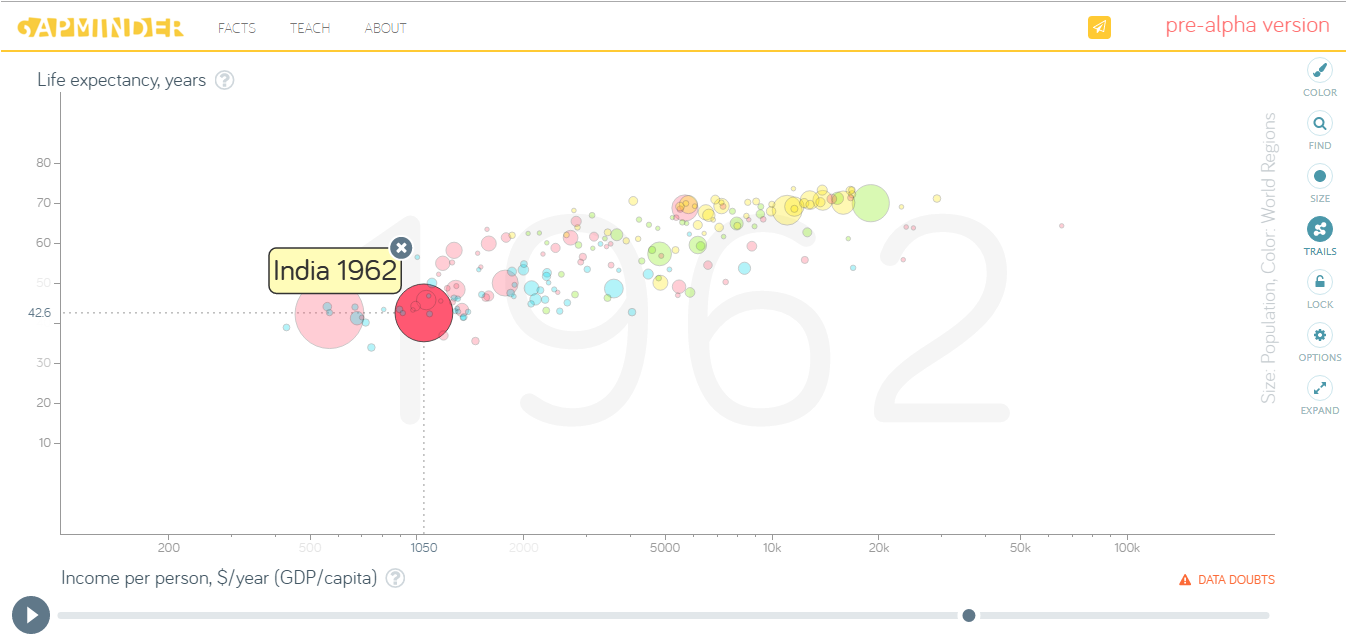
\includegraphics[scale=.4]{image/gapminder}
    \caption{Đồ thị trực quan dữ liệu Gapminder World}
    \label{refhinh1}
\end{figure}

Như ở hình 1, chúng ta có thể thấy với 1 lượng dữ liệu lớn (ở đây là độ tuổi kỳ vọng ở các quốc gia trên thế giới), có thể được thể hiện trực quan bởi đồ thị bong bóng (bubble chart). Qua kích thước các bong bóng, có thể thấy sự tương quan khác biệt giữa các quốc gia như thế nào. Hay khi trỏ vào 1 bong bóng, chúng ta thấy được số liệu chi tiết ở quốc gia đó, như trong hình là độ tuổi kỳ vọng ở Ấn Độ, vào năm 1962 là 42.6. Ngoài ra ở phía dưới đồ thị, có 1 thanh thể hiện dòng thời gian (timeline), khi thanh thời gian trượt đi, kích thước các quả bóng thay đổi theo như số liệu tương ứng ở các năm của các quốc gia.



\subsubsection{Phương pháp}
Gapminder sử dụng D3.js, một thư việc JavaScript phổ biến trong việc thao tác với các thành phần của một trang web (Document Object Model) dựa trên dữ liệu. 

D3 cho phép thể hiện dữ liệu thông qua HTML, SVG và CSS. D3 còn là một tiêu chuẩn web cung cấp hầu hết các khả năng mà một trình duyệt hiện đại mang lại, mà không cần phải tự viết lại hay dựa trên một nền tảng khuôn khổ. Kết hợp các thành phần trực quan mạnh mẽ và hướng tiếp cận dữ liệu để thao tác trên DOM.

\subsubsection{Đánh giá}
Với mục tiêu luôn luôn cập nhật các công cụ cũng như dữ liệu, nhằm đảm bảo tính xác thực, và đúng đắn của ứng dụng, Gapminder World đảm bảo nguồn dữ liệu chính xác nhất và cập nhật nhất.
Dữ liệu đề tài sẽ sử dụng từ Gapminder để đảm bảo nguồn thông tin luôn xác thực và thể hiện đúng đắn nhất các xu hướng phát triển toàn cầu.

Ngoài ra, cách sử dụng các biểu đồ con để hiển thị dữ liệu liên quan của một đối tượng được tương tác giúp người dùng dễ dàng nắm bắt được chính xác các thông tin muốn truyền đạt, tăng tính thân thiện cũng như trải nghiệm người dùng. Áp dụng tính hiệu quả trên, đề tài đề xuất sử dụng cách thể hiện trải nghiệm người dùng (UI/UX) kế thừa các đặc tính của Gapminder World. 

Về thư viện D3.js được sử dụng trong Gapminder World, đây là một thư viện mạnh mẽ tiếp cận dữ liệu dựa trên các thao tác với DOM. D3.js cho phép tái sử dụng các thành phần và trình nhúng (plugin) một cách đơn giản và hiệu quả. Đề tài đề xuất sử dụng D3.js làm thư viện chính để hiện thực thư viện tương tác giữa các đồ thị.

\subsection{Global Health Atlas - WHO}
\subsubsection{Giới thiệu}
Trong một môi trường điện tử, WHO’s Communicable Disease Global Atlas được dùng cho việc phân tích và so sánh dữ liệu chuẩn, thống kê các bệnh truyền nhiễm ở các quốc gia, vùng lãnh thổ, và toàn thế giới. Việc phân tích và biểu diễn dữ liệu ngày càng được hỗ trợ tốt hơn thông qua các thông tin về dân số, điều kiện kinh tế xã hội, và các yếu tố môi trường. Với việc làm đó, Atlas có thể biết được những yếu tố gây ra bệnh truyền nhiễm.

\begin{center}
    \begin{figure}[htp]
    \begin{center}
     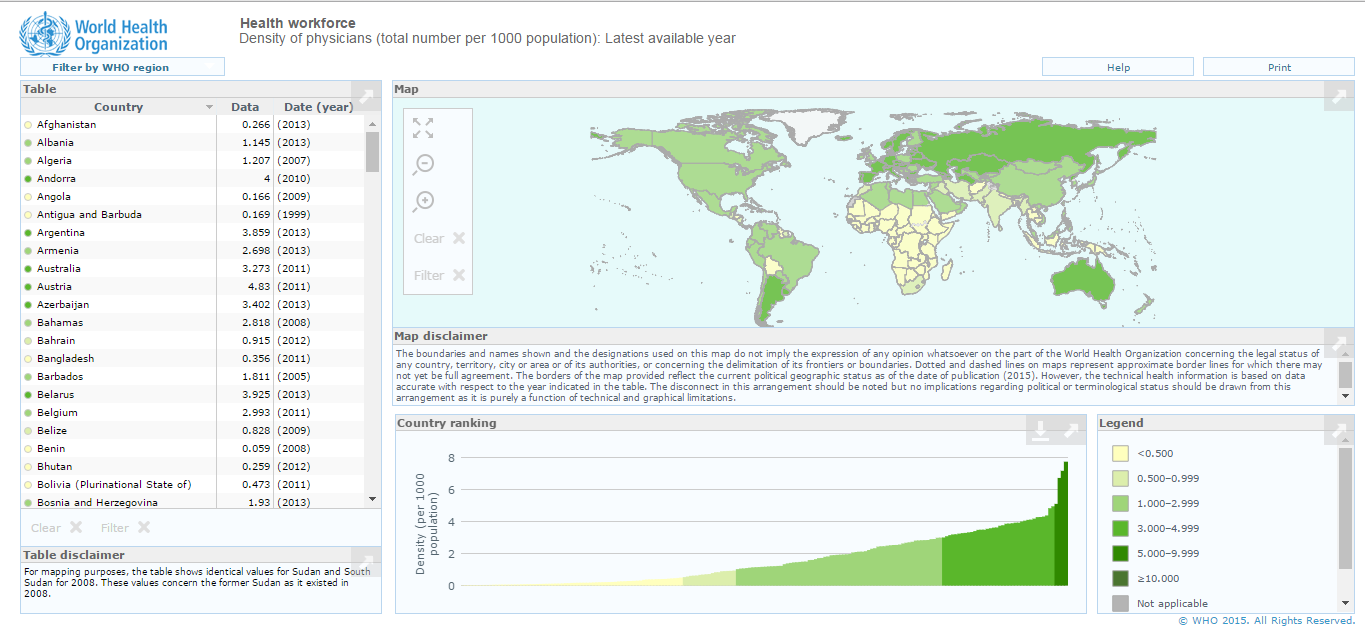
\includegraphics[scale=.4]{image/globalatlas}
    \end{center}
    \caption{Biểu đồ tương tác về mật độ bác sĩ của WHO}
    \label{refhinh2}
    \end{figure}
\end{center}

\subsubsection{Mục tiêu}
Ban đầu, với mục đích cung cấp những dữ liệu, báo cáo về các bệnh truyền nhiễm chính (sốt rét, HIV/AIDS,..), thì ngày nay Global Atlas của WHO cũng dùng để phân tích, biểu diễn, so sánh dữ liệu từ những vấn đề liên quan đến y tế khác như: mật độ bác sĩ, số lượng người chết do tai nạn giao thông, tuổi thọ trung bình,… 

\subsubsection{Phương pháp}
Trực quan dữ liệu thành nhiều dạng biểu đồ khác nhau, các biểu đồ có thể tương tác với nhau giúp cho việc nhìn nhận, phân tích, đánh giá thông tin một cách chính xác, đầy đủ.

Ứng dụng bao gồm các thành phần:

\indent \indent \textbullet \ Bảng dữ liệu: được lấy từ database của WHO

\indent \indent \textbullet \ Map: dùng thư viện Google Maps, kết hợp với bảng dữ liệu để tạo ra biểu đồ

\indent \indent \textbullet \ Biểu đồ cột: dựa vào bảng dữ liệu để tạo ra biểu đồ

\indent \indent \textbullet \ Chú thích: phân vùng dữ liệu

Tính năng: ứng dụng hỗ trợ tương tác giữa các biểu đồ, bảng dữ liệu:

\indent \indent \textbullet \ Khi click vào 1 hàng trong bảng dữ liệu, bên map sẽ phóng to đến vùng tương ứng, bên biểu đồ cột sẽ nổi bật cột tương ứng. Các tương tác sẽ được thể hiện tương tự khi click vào các biểu đồ.
\begin{center}
    \begin{figure}[htp]
    \begin{center}
     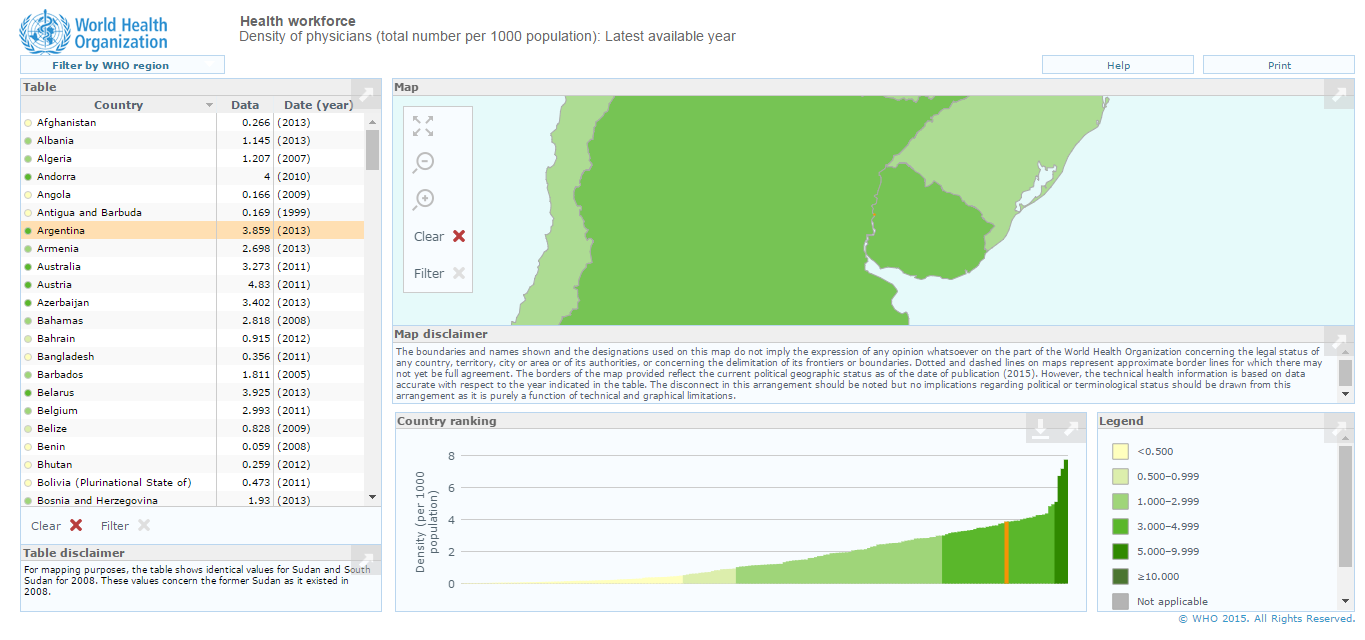
\includegraphics[scale=.4]{image/clickatlas}
    \end{center}
    \caption{Tương tác khi click vào một hàng trong bảng dữ liệu}
    \label{refhinh3}
    \end{figure}
\end{center}
\indent \indent \textbullet \ Khi hover lên 1 hàng trong bảng dữ liệu, bên các biểu đồ cũng sẽ được làm nổi bật vùng tương ứng như khi click, nhưng với 1 màu sắc khác (bên map sẽ không phóng to đến vùng tương ứng).
\begin{center}
    \begin{figure}[htp]
    \begin{center}
     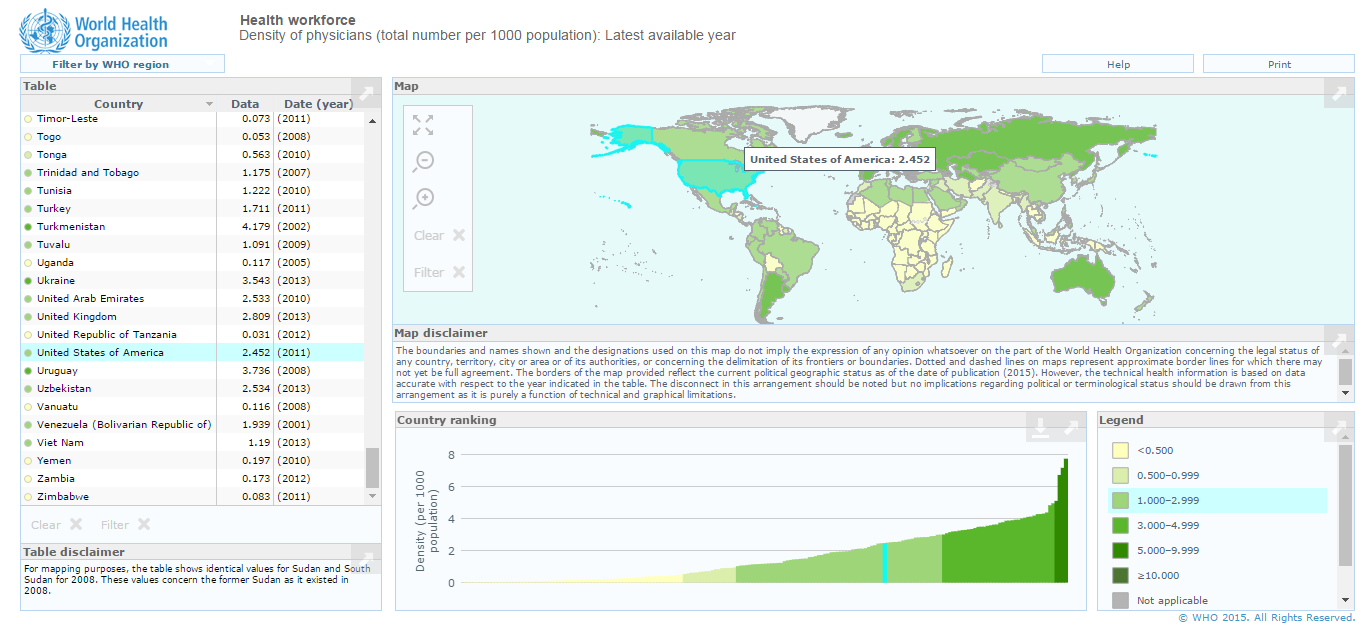
\includegraphics[scale=.4]{image/hoveratlas}
    \end{center}
    \caption{Tương tác khi hover lên Map}
    \label{refhinh4}
    \end{figure}
\end{center}
\subsubsection{Đánh giá}
Dữ liệu được WHO thu thập trên toàn thế giới, cập nhật theo thời gian, đảm bảo tính chính xác của ứng dụng.

Bên cạnh đó, việc trực quan thành nhiều loại biểu đồ, thể hiện được nhiều cái nhìn khác nhau của dữ liệu giúp đánh giá vấn đề 1 cách đúng đắn, đầy đủ.

Một tính năng khác đó là việc tương tác giữa các giữa các đồ thị giúp người dùng có nhiều cái nhìn từ nguồn dữ liệu, hiểu được thông tin rút trích từ các đồ thị, tăng tính thân thiện, trải nghiệm của người dùng.

Do đó, đề tài đề xuất sử dụng nhiều đồ thị để biểu diễn cho nguồn dữ liệu đầu vào, và sự tương tác giữa các đồ thị.

\subsection{Thư viện đồ thị C3.js}
\subsubsection{Giới thiệu}
C3.js là một thư viện mã nguồn mở [link c3js.org] dựa trên thư viện D3.js , nhằm cho phép người dùng có cái nhìn sâu hơn về các ứng dụng web tích hợp đồ thị.

Toàn bộ mã nguồn của thư viện nằm ở: https://github.com/masayuki0812/c3
\begin{figure}[htp]
    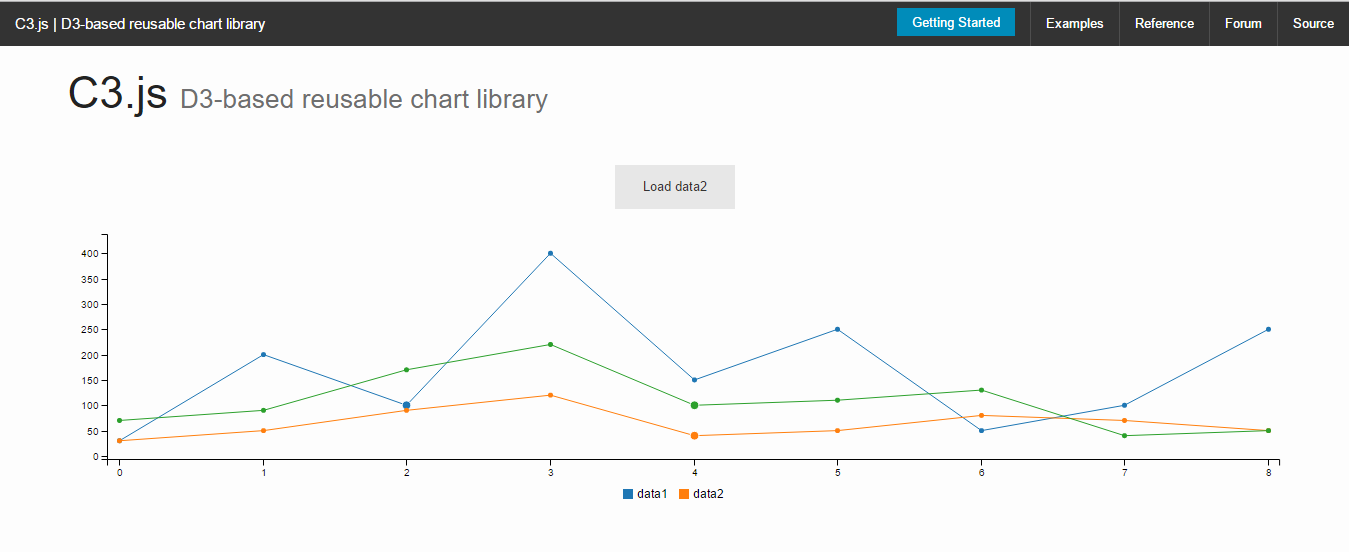
\includegraphics[scale=.4]{image/c3js}
    \caption{Thư viện đồ thị C3js}
    \label{refhinh5}
\end{figure}

\subsubsection{Mục tiêu}
\begin{itemize}
        \item[•]Sự thoải mái (Comfortable)
        C3 giúp người dùng có thể dễ dàng tạo một đồ thị dựa trên D3 bằng cách gộp chung các đoạn code cần thiết để cấu trúc một đồ thị hoàn chỉnh. Qua đó, người dùng không cần phải viết các đoạn code D3 rườm rà như trước nữa.
\begin{figure}[htp]
    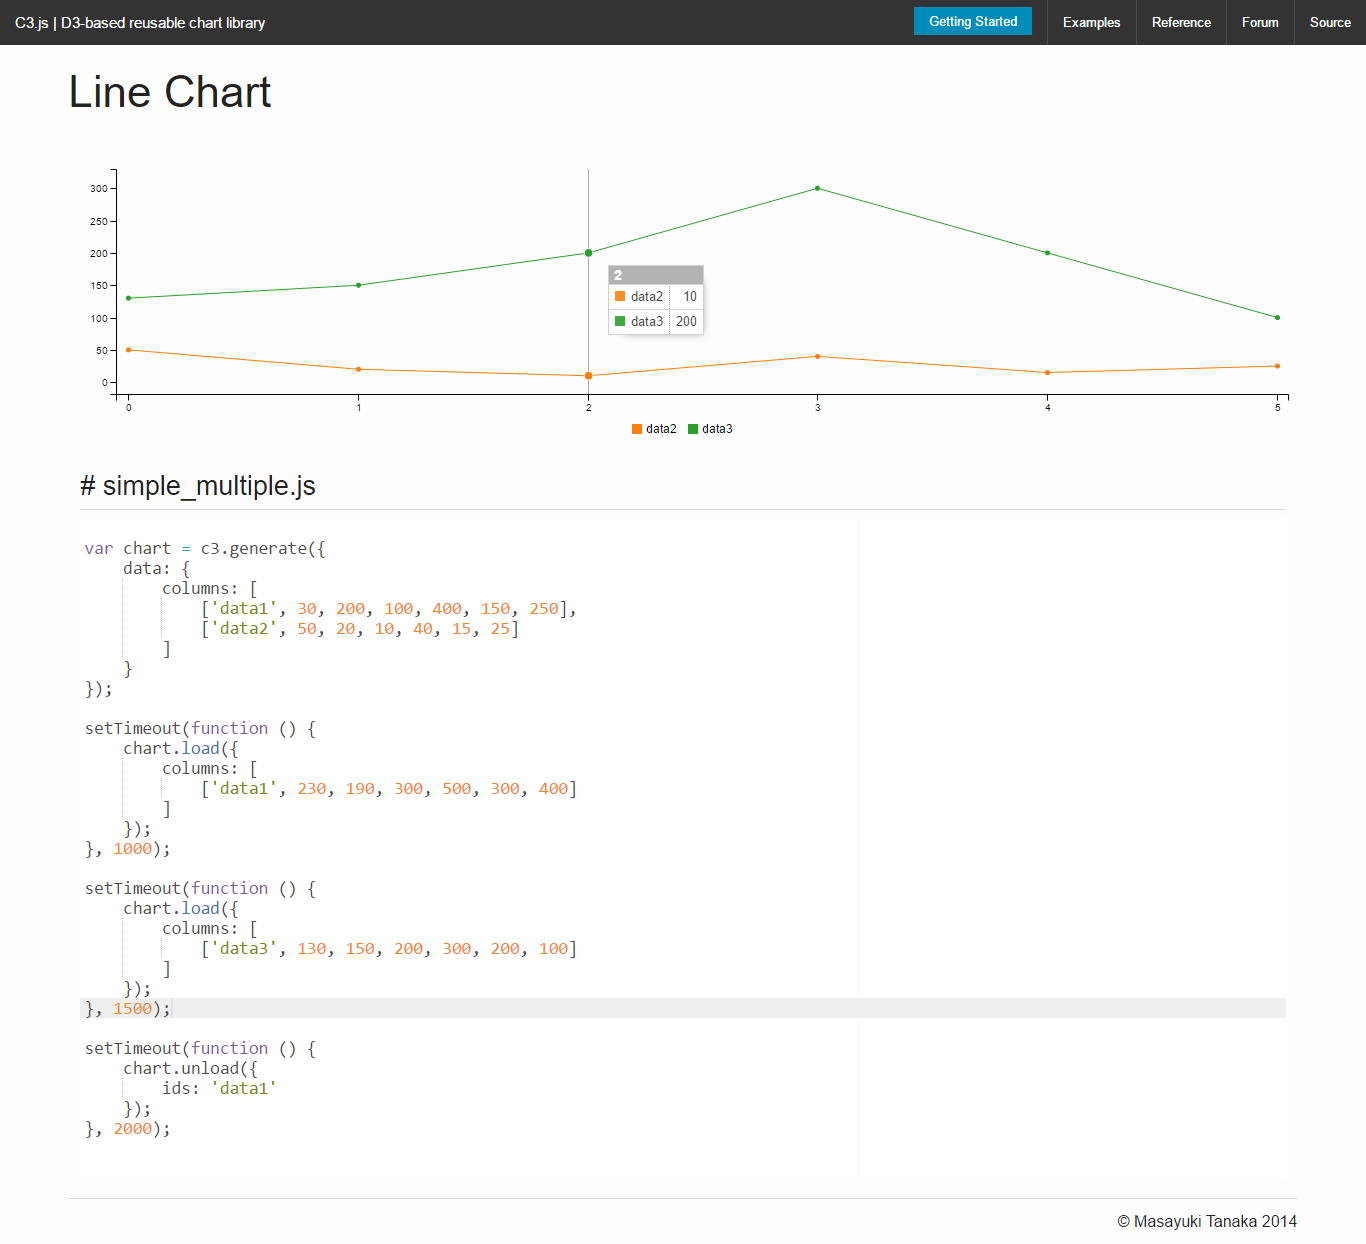
\includegraphics[scale=.3]{image/c3syntax}
    \caption{Thư viện đồ thị C3js}
    \label{refhinh6}
\end{figure}
[Hình 6] Thông qua một số câu lệnh định nghĩa dữ liệu, C3 khởi tạo một đồ thị cho phép tương tác một cách trực quan thông qua hover, click,.. các thành phần của đồ thị

        \item[•]Khả năng tuỳ chỉnh (Customizable)
        C3 cung cấp các class tương ứng cho mỗi đối tượng trong đồ thị khi khởi tạo. Qua đó, người dùng có thể định nghĩa các style theo ý muốn theo class cũng như mở rộng cấu trúc các thành phần của đồ thị (trục dữ liệu, hình dạng hiển thị, kiểu đồ thị,.. ) một cách trực tiếp.
\begin{figure}[htp]
    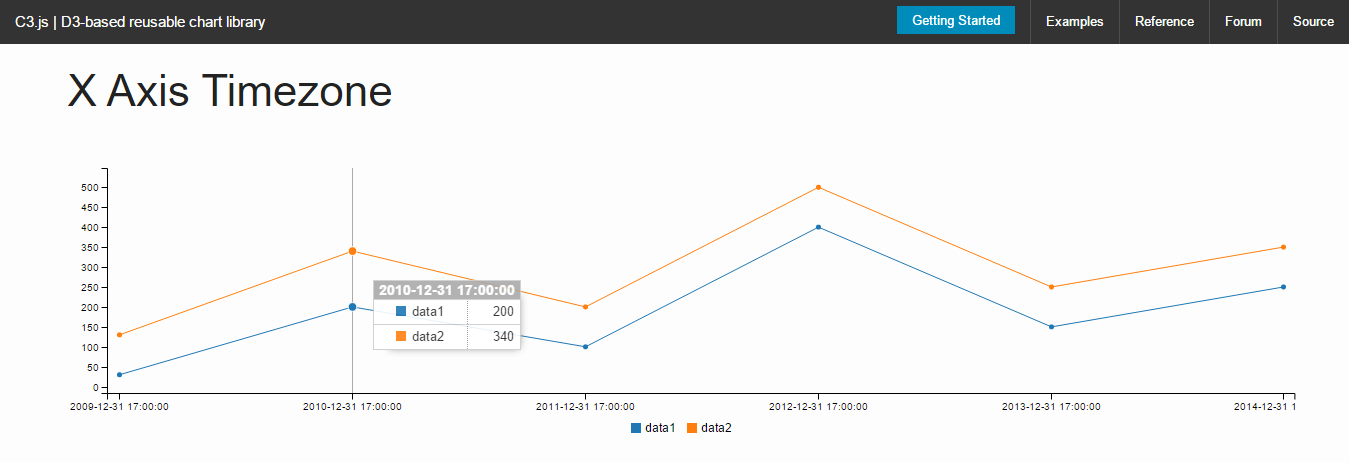
\includegraphics[scale=.4]{image/c3custom}
    \caption{Thư viện đồ thị C3js}
    \label{refhinh7}
\end{figure}      
[Hình 7] Trục hoành của đồ thị được tuỳ chỉnh theo thời gian hiện tại với định dạng hoàn toàn tuỳ thuộc người sử dụng.
 
        \item[•]Khả năng kiểm soát (Controllable)
        C3 cung cấp đa dạng các APIs và các hàm callback để truy xuất trạng thái của đồ thị. Bằng cách đó, người dùng có thể cập nhật lại đồ thị thậm chí sau khi đồ thị đã được thể hiện.
\begin{figure}[htp]
    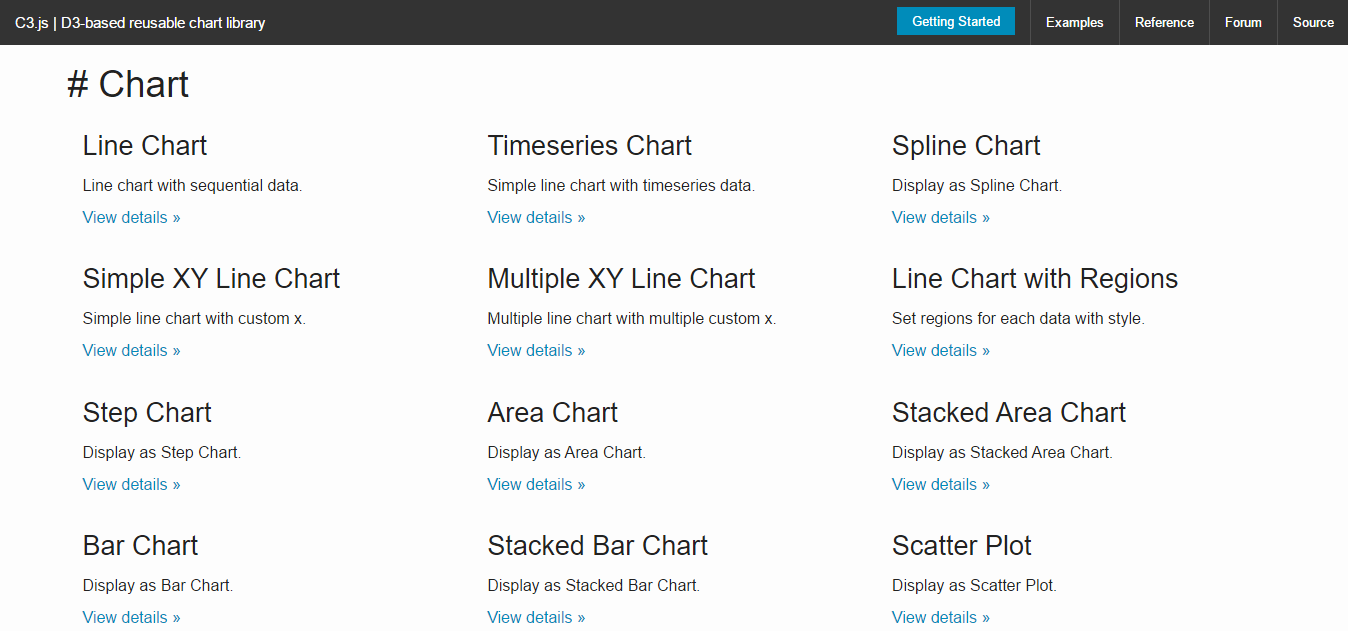
\includegraphics[scale=.4]{image/c3apis}
    \caption{Thư viện đồ thị C3js}
    \label{refhinh8}
\end{figure}
[Hình 8] Trên hình là một số các thành phần được hỗ trợ bởi thư viện C3js
\end{itemize}

\subsubsection{Phương pháp}
Như đã trình bày ở trên, C3js sử dụng thư viện D3js nhằm tạo các đồ thị có khả năng tái sử dụng, cũng như giúp người dùng đào sâu hơn vào khái niệm trực quan dữ liệu thông qua đồ thị trên nền ứng dụng web.

Ngoài ra dựa theo cấu trúc mã nguồn mà C3js chia sẻ, có thể thấy cấu trúc tổ chức của C3js theo hướng hướng đối tượng, được tổ chức theo các class (trục, dữ liệu, đồ thị,.. ) và các phương thức, thuộc tính đi kèm class.

\begin{figure}[htp]
    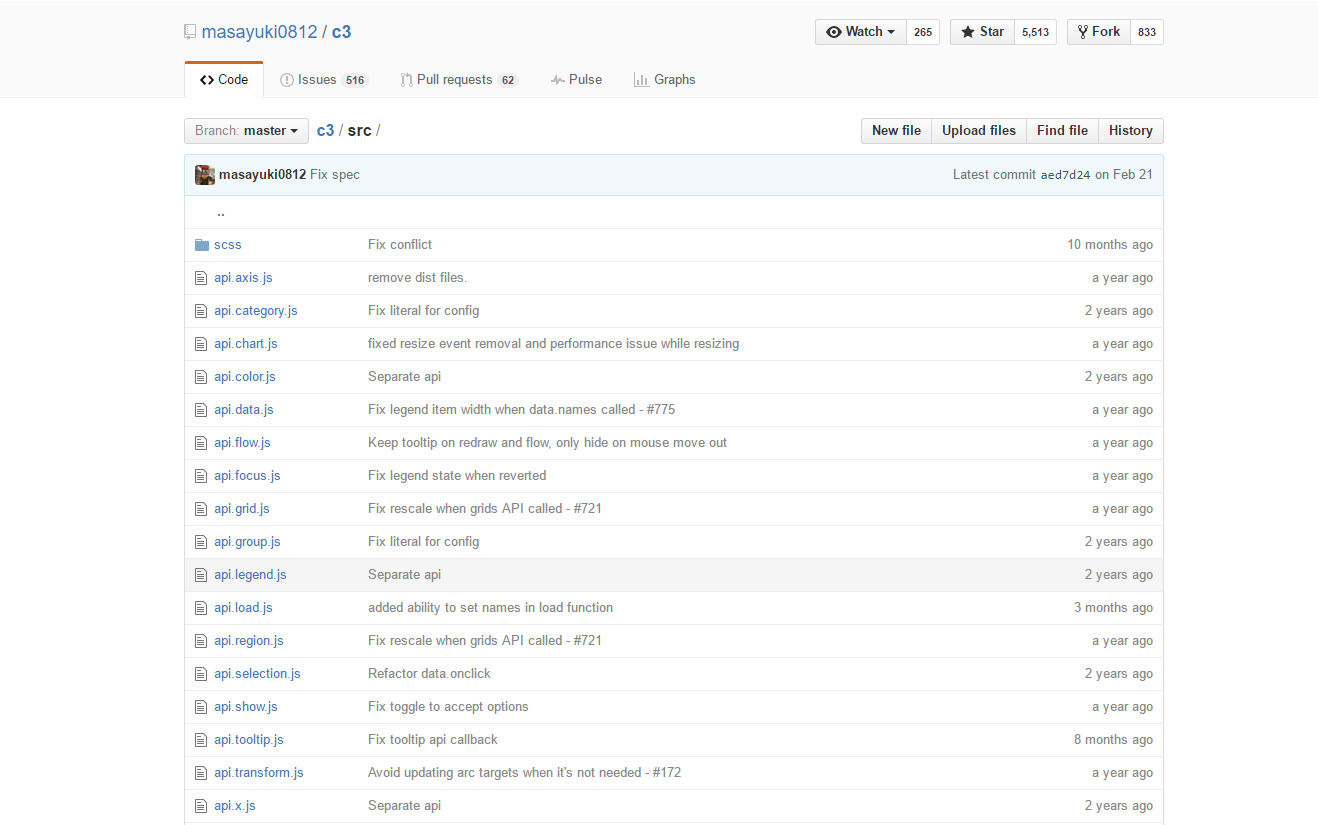
\includegraphics[scale=.4]{image/c3source}
    \caption{Thư viện đồ thị C3js}
    \label{refhinh9}
\end{figure}

\subsubsection{Đánh giá}
Cách tổ chức và hiện thực theo hướng hướng đối tượng như trên giúp tiết kiệm số dòng mã, tận dụng khả năng tái sử dụng, đồng thời giúp việc mở rộng về sau rất hiệu quả.

Đề tài đề xuất sử dụng cách hiện thực API theo hướng như C3js.

\subsection{Ứng dụng tạo bản đồ online Mapme}
\subsubsection{Giới thiệu}
Mapme là một ứng dụng cho phép người dùng tạo bản đồ, dữ liệu đươc xử lý trực tiếp từ các file Excel đầu vào. Bản đồ tạo ra có các marker tương ứng với dữ liệu, có khả năng tương tác trực tiếp thông qua các sự kiện định nghĩa trước. Ngoài ra, bản đồ được tạo ra còn có thể được nhúng vào các trang web khác thông qua một đoạn mã nhúng. Đặc biệt toàn bộ tương tác từ những bước khởi tạo bản đồ đầu tiên, đến lúc xuất thành quả, đều không yêu cầu người dùng phải viết một dòng mã nào.

\begin{figure}[htp]
    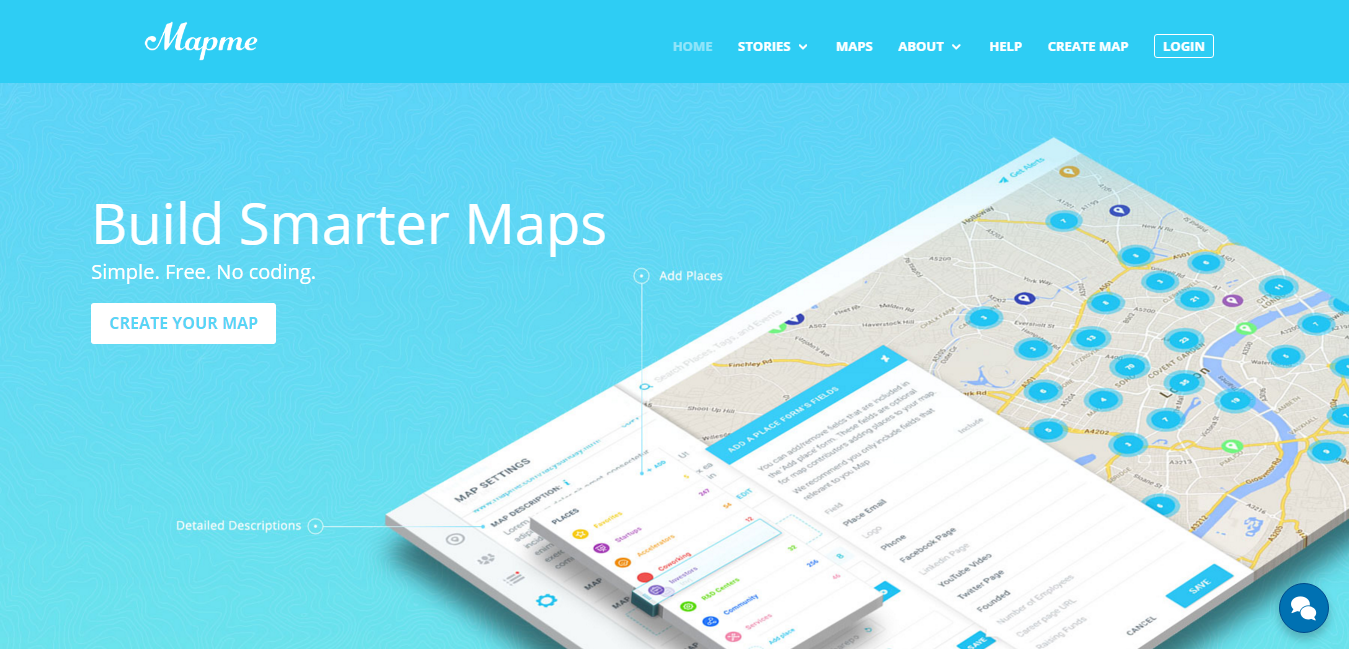
\includegraphics[scale=.4]{image/mapme}
    \caption{Ứng dụng tạo bản đồ online Mapme}
    \label{refhinh10}
\end{figure}

\subsubsection{Mục tiêu}
Đầu tiên nói đến các đối tượng mà Mapme hướng tới, đó là các tổ chức, chính phủ, các doanh nghiệp hay các tổ chức cộng đồng phi lợi nhuận.

Phục vụ trong các lĩnh vực khác nhau như giáo dục, các sự kiện, xuất bản hay truyền thụ cảm hứng trong đời sống hằng ngày.

\subsubsection{Phương pháp}
Sử dụng OpenStreetMap (viết tắt OSM), một dịch vụ bản đồ thế giới trực tuyến với nội dung mở, được bảo trợ bởi các công ty lớn như Google, Yahoo! và Multimap.com. OSM cho phép ứng dụng cập nhật dữ liệu địa lý trực tuyến một cách chính xác, luôn được cập nhật nhằm đảm bảo các dữ liệu luôn đi xát thực tế nhất.

\begin{figure}[htp]
    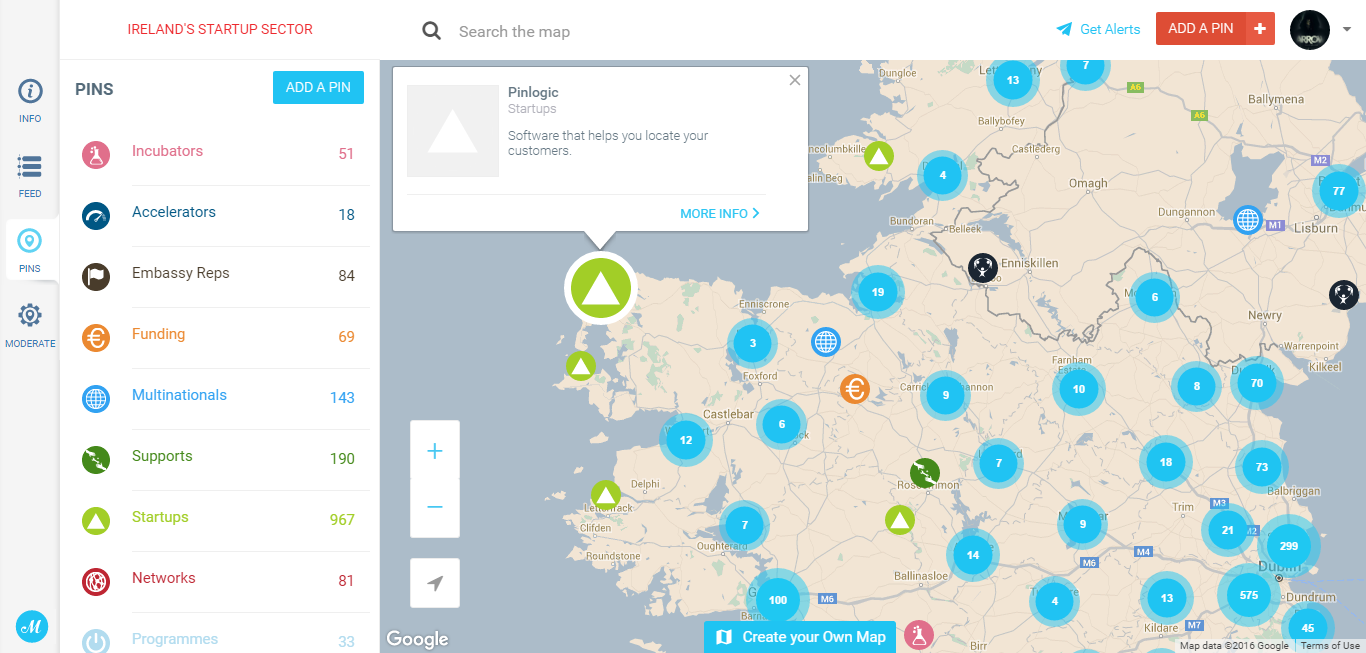
\includegraphics[scale=.4]{image/mapmeOSM}
    \caption{Ứng dụng tạo bản đồ online Mapme}
    \label{refhinh11}
\end{figure}

Như trên hình có thể thấy, các thông tin về khởi nghiệp ở quốc gia Ireland được trực quan thông qua các biểu tượng (marker). Cùng với đó là các số liệu tương ứng được xử lý trực tiếp từ các file Excel đầu vào.
Ngoài ra, người dùng còn có thể tương tác với các marker này để thể hiện thông tin chi tiết ở các điểm chỉ định.

\begin{figure}[htp]
    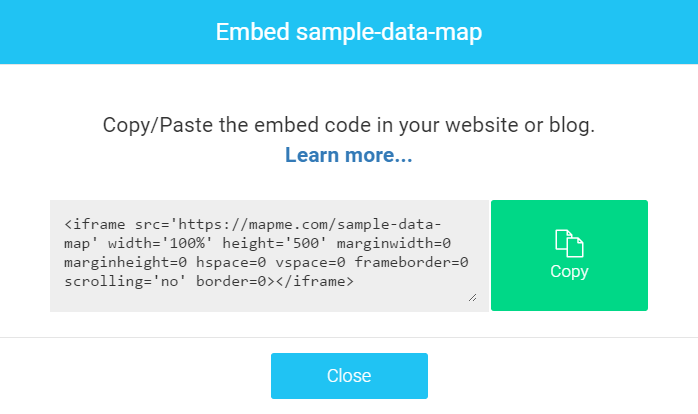
\includegraphics[scale=.8]{image/mapmeExport}
    \caption{Ứng dụng tạo bản đồ online Mapme}
    \label{refhinh12}
\end{figure}

Đặc biệt, Mapme còn hỗ trợ sinh mã nhúng, dưới dạng iframe, giúp người dùng nhúng trực tiếp bản đồ mình vừa tạo vào các website tuỳ mục đích.

\subsubsection{Đánh giá}
Đầu tiên là về cách sử dụng OpenStreetMap làm dịch vụ cung cấp bản đồ, đảm bảo ứng dụng luôn chính xác về các dữ liệu địa lý so với thực tế. Đề tài đề xuất sử dụng OpenStreetMap làm dịch vụ cung cấp bản đồ cho API mà đề tài thực hiện.

Ngoài ra, ứng dụng cho phép người dùng tương tác trực tiếp với các marker trên bản đồ, hiển thị các thông tin liên quan đến các địa điểm đó. Thay vì phải đọc các dữ liệu thô theo vùng miền, theo quốc gia, vùng lãnh thổ như trước, cách tương tác này giúp người dùng dễ dàng cập nhật thông tin cũng như có cái nhìn tổng quan, khả năng so sánh giữa các địa điểm khác nhau mà không phải chăm chú vào các con số nhàm chám như trước.

\section{Kiến thức nền}
Qua việc tìm hiểu cũng như những phần trình bày về các công trình liên quan đến đề tài, đề tài nhận thấy cần phải nắm được những kiến thức cơ bản sau để hỗ trợ tốt hơn cho việc hiện thực API về trực quan dữ liệu:
\subsection{Javascript}
\subsubsection{Giới thiệu}
JavaScript, theo phiên bản hiện hành, là một ngôn ngữ lập trình kịch bản (scripting language), đa nền tảng (cross-platform), nhỏ và nhẹ. Ngôn ngữ này được dùng rộng rãi cho các trang web, nhưng cũng được dùng để tạo khả năng viết script sử dụng các đối tượng nằm sẵn trong các ứng dụng.

\subsubsection{Mục tiêu}
Mục tiêu của JavaScript là nhằm cung cấp cho các nhà phát triển Web một số khả năng và quyền điều khiển chức năng cho trang Web. Mã Javascript có khả năng nhúng trong tài liệu HTML để điều khiển nội dung của trang Web và kiểm tra sự hợp lệ của dữ liệu mà người dùng nhập vào. Khi một trang hiển thị trong trình duyệt, các câu lệnh được trình duyệt thông dịch và thực thi.

\subsubsection{Tính năng}
JavaScript nâng cao tính động và khả năng tương tác cho web-site bằng cách sử dụng các hiệu ứng của nó như thực hiện các phép tính, kiểm tra form, viết các trò chơi, bổ sung các hiệu ứng đặc biệt, tuỳ biến các chọn lựa đồ hoạ, tạo ra các mật khẩu bảo mật và hơn thế nữa.

Cụ thể, Javascript có thể được dùng để:
 
\indent \indent \textbullet \ Tương tác với người dùng, chúng ta có thể viết mã để đáp lại các sự kiện. Các sự kiện này sẽ có thể phát sinh bởi người dùng: nhấp chuột hay được phát sinh từ hệ thống, định lại kích thước của trang …

\indent \indent \textbullet \ Thay đổi nội dung động. Mã JavaScript có thể dùng để thay đổi nội dung và vị trí các phần tử một cách động trên một trang nhằm đáp lại sự tương tác với người dùng.

\indent \indent \textbullet \ Kiểm tra tính hợp lệ dữ liệu. Chúng ta có thể viết mã nhằm kiểm tra tính hợp lệ của dữ liệu do người dùng nhập vào trước khi nó được gửi lên Web server để xử lý.

\subsubsection{Ứng dụng}


\subsection{jQuery}
\subsubsection{Giới thiệu}
jQuery là một thư viện đa nền tảng (cross-platform) mã nguồn mở dựa trên ngôn ngữ Javascript, được tạo bởi John Resig vào năm 2006. jQuery. jQuery là một thư viện Javascript phổ biến nhất được sử dụng hiện nay.

Theo thống kê (link: http://w3techs.com/technologies/details/js-jquery/all/all), cho tới hiện nay thì jQuery được sử dụng bởi 96\% của tất cả các trang web có sử dụng thư viện Javascript.

\subsubsection{Mục tiêu}
Với phương châm là “write less, do more”, jQuery được thiết kế nhằm đơn giản hóa các nhiệm vụ khác nhau bằng cách viết ít mã hơn. 

Thành phần quan trọng của jQuery là thư viện thao tác DOM (Document Object Model). DOM là 1 biểu diễn cấu trúc cây của tất cả các thành phần của 1 trang web và jQuery đơn giản hóa các cú pháp cho việc tìm kiếm, chọn lựa, và thao tác những phần tử DOM.

\subsubsection{Tính năng}
\indent \indent \textbullet \ Việc lựa chọn các phần tử DOM sử dụng công cụ Sizzle (selector mã nguồn mở)

\indent \textbullet \ Thao tác với DOM dựa trên CSS Selector

\indent \textbullet \ Sư kiện (event)

\indent \textbullet \ Tạo chuyển động

\indent \textbullet \ Hỗ trợ AJAX

\indent \textbullet \ Có thể mở rộng thông qua các plug-in

\indent \textbullet \ Được hỗ trợ bởi nhiều trình duyệt

\indent \textbullet \ Cập nhật và hỗ trợ các công nghệ web mới nhất (HTML5 \& CSS3)

\begin{center}
    \begin{figure}[htp]
    \begin{center}
     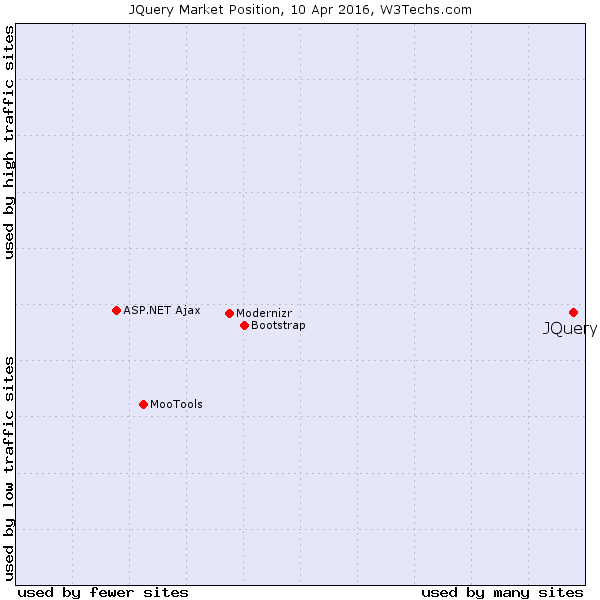
\includegraphics[scale=.6]{image/js-jquery}
    \end{center}
    \caption{Vị trí của jQuery so với những thư viện Javascript khác}
    \label{refhinh13}
    \end{figure}
\end{center}

\subsubsection{Ứng dụng}
Dựa trên những đặc điểm cũng như tính năng mạnh mẽ của jQuery nói trên, đề tài sẽ đề xuất sử dụng jQuery như là 1 ngôn ngữ chính, tạo ra một API dễ dàng tìm hiểu, sử dụng với một số lượng mã (code) ít nhất để có thể tạo được ứng dụng của riêng mình.

\subsection{d3.js}
\subsubsection{Giới thiệu}
D3.js được viết bởi Mike Bostock, là 1 thư viện javascript dùng để thao tác với document dựa trên dữ liệu (data). D3 giúp mang dữ liệu đến cuộc sống bằng cách sử dụng HTML, SVG, và CSS. D3 trên chuẩn web cung cấp đầy đủ các tính năng của những trình duyệt hiện đại mà không buộc mình vào một khuôn khổ nhất định nào, kết hợp với các thành phần trực quan mạnh mẽ và một phương pháp hướng dữ liệu để thao tác DOM.

\begin{center}
    \begin{figure}[htp]
    \begin{center}
     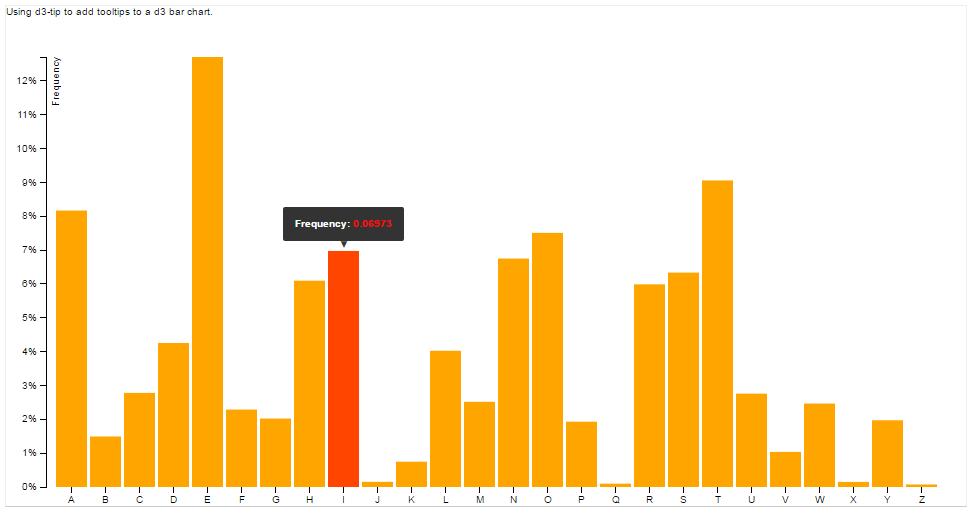
\includegraphics[scale=.6]{image/d3}
    \end{center}
    \caption{Một ví dụ về d3.js}
    \label{refhinh14}
    \end{figure}
\end{center}

\subsubsection{Mục tiêu}
D3.js giúp nhúng dữ liệu vào trong các phần tử DOM. Sau đó, có thể áp dụng CSS3, HTML, và/hoặc SVG lên dữ liệu này. Cuối cùng, D3.js có thể giúp tạo ra dữ liệu tương tác thông qua việc sử dụng những sự biến đổi (transformation), chuyển đổi (transition) hướng dữ liệu của D3.js

\subsubsection{Ứng dụng}
D3.js được viết trong Javascript, do đó có thể sử dụng lại code và thêm những hàm chức năng mà người dùng muốn. Cách người dùng chọn để định dạng, thao tác, tương tác với dữ liệu là tùy thuộc ở họ.

D3.js rất thích hợp dùng trong đề tài, nó giúp xây dựng framework trực quan dữ liệu mà người dùng muốn, dễ dàng sử dụng, do đó giúp tạo ra API một cách dễ dàng hơn, API dễ hiểu, dễ sử dụng.

\subsection{OpenLayers}
\subsubsection{Giới thiệu}
OpenLayers được tạo ra bởi MetaCarta sau hội nghị O'Reilly Where 2.0 (29-30/06/2005) và chính thức phát hành thành mã nguồn mở trước hội nghị  O'Reilly Where 2.0 (13-14/06/2006) bởi MetaCarta Labs. Hai dự án khác về công cụ xây dựng bản đồ phát hành bởi MetaCarta là FeatureServer và TileCache. Từ tháng 11/2007, OpenLayers trở thành dự án mã nguồn mở chính thức của Hội đồng Không gian địa lý.

Sơ qua về OpenLayers, đây là một thư viện JavaScript mã nguồn mở (được chứng nhận bởi BSD License) nhằm phục vụ mục đích biểu diễn thông tin trên bản đồ  đối với các trình duyệt Web, không phụ thuộc phía server. Nó cung cấp API chuyên về xây dựng các ứng dụng địa lý trên nền Web tương tự như Google Maps[link] và Bing Maps[link], với một điểm khác biệt duy nhất, OpenLayers hoàn toàn miễn phí, được xây dựng và phát triển nên bởi cộng đồng phát triển phần mềm mã nguồn mở. Thư viện xây dựng trên Prototype JavaScript Framework [link].

Hiện nay, OpenLayers đã ra tới phiên bản OpenLayers 3[link]. OpenLayers 3 được viết lại nhằm dễ hiểu hơn, hướng tới các tính năng của HTML5 và CSS3. Thư viện tiếp tục hỗ trợ trình chiếu, các giao thức tiêu chuẩn và các chức năng chỉnh sửa. Phiên bản mới này tập trung vào cải thiện hiệu năng, xây dựng đơn giản hơn, các thành phần trở nên trực quan hơn, API được cải tiến và còn nhiều hơn nữa.

Source code của thư viện: \href{https://github.com/openlayers/ol3/}{https://github.com/openlayers/ol3/}

\subsubsection{Mục tiêu}
Như đã trình bày ở trên, OpenLayers hỗ trợ các lập trình viên hiển thị thông tin dưới dạng bản đồ, hay bất cứ nhu cầu nào liên quan về bản đồ một cách hiệu quả và đơn giản nhất.

\subsubsection{Đặc điểm}
	\begin{center}
    	\begin{figure}[htp]
    		\begin{center}
     		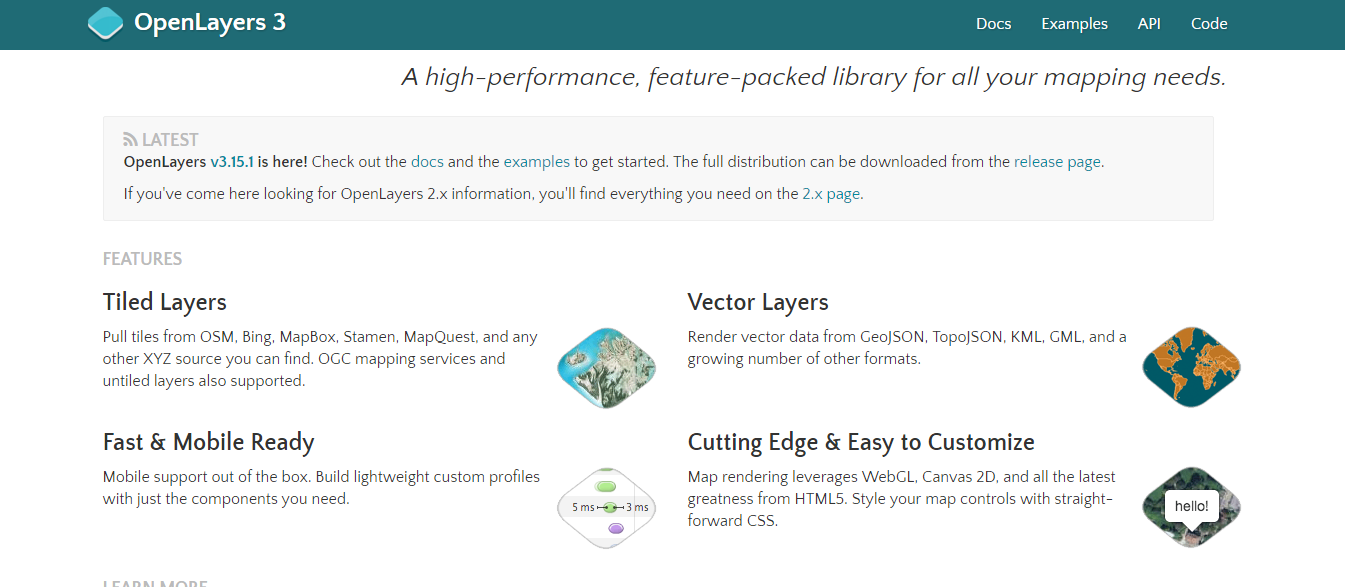
\includegraphics[scale=.4]{image/ol-feature}
    		\end{center}
    	\caption{Các đặc điểm chính của OpenLayers}
    	\label{refhinh15}
    	\end{figure}
	\end{center}
OpenLayers có 4 đặc điểm chính:
\begin{itemize}
\item[•]Thể hiện Lớp dưới dạng ô (Tiled Layers): 
Các lớp này được kéo về từ OpenStreetMap (OSM), Bing, MapBox, Stamen, MapQuest và bất cứ nguồn nào mà bạn có thể tìm thấy. Hỗ trợ đa dạng các Layer mà bạn có thể sử dụng trong ứng dụng của mình.

\item[•]Thể hiện Lớp dưới dạng Vector (Vector Layers):
Sinh ra dữ liệu dạng vector từ GeoJSON, TopoJSON, KML, GML và một số định dạng khác.

\item[•]Tính đối ứng nhanh gọn (Fast \& Mobile Ready):
Hỗ trợ tùy chỉnh các thành phần một cách nhanh gọn và thuận tiện nhất. Cho phép xây dựng một bản tùy chỉnh gọn nhẹ gồm các thành phần mà lập trình viên cần.

\item[•]Mài dũa các góc cạnh và dễ dàng tùy chỉnh (Cutting Edge \& Easy to Customize):
Bản đồ sinh ra bởi công nghệ WebGL, Canvas 2D, và từ những tính năng ưu việt nhất của HTML5. Dễ dàng tùy chỉnh style bằng CSS.

\end{itemize}

\subsubsection{Ứng dụng}
Đề tài hướng tới xây dựng thư viện JavaScript cho phép tương tác giữa bản đồ và các đồ thị dựa trên dữ liệu đầu vào, cho nên OpenLayers, cụ thể OpenLayers 3 sẽ là công cụ đắc lực cho việc xây dựng thành phần bản đồ trong đề tài. 


\section{Giải pháp đề xuất}

\section{Kế hoạch thực hiện}
\end{document}
